\documentclass[tikz,border=2pt]{standalone}
\usepackage{amsmath,amssymb}
\usepackage{tikz}
\usetikzlibrary{matrix,arrows.meta}

\begin{document}
% Three agents but only two tasks: add a dummy task column of zero costs to make the matrix
% square; the agent assigned to the dummy task simply gets nothing to do.
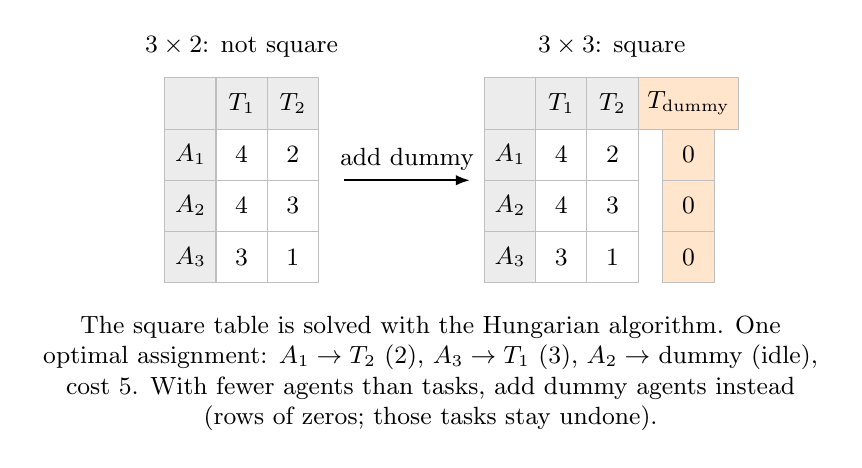
\begin{tikzpicture}[every node/.style={font=\small}, >={Latex[length=1.8mm]}]
	\matrix (A) [matrix of math nodes, nodes={minimum size=6.5mm, anchor=center, draw=gray!50}, column sep=-\pgflinewidth, row sep=-\pgflinewidth] at (0,0) {|[fill=gray!15]| & |[fill=gray!15]| T_1 & |[fill=gray!15]| T_2 \\ |[fill=gray!15]| A_1 & 4 & 2 \\ |[fill=gray!15]| A_2 & 4 & 3 \\ |[fill=gray!15]| A_3 & 3 & 1 \\};
	\node[anchor=south] at (A.north) {$3\times2$: not square};
	\draw[->, thick] (1.3,0) -- (2.9,0) node[midway, above] {add dummy};
	\matrix (B) [matrix of math nodes, nodes={minimum size=6.5mm, anchor=center, draw=gray!50}, column sep=-\pgflinewidth, row sep=-\pgflinewidth] at (4.7,0) {|[fill=gray!15]| & |[fill=gray!15]| T_1 & |[fill=gray!15]| T_2 & |[fill=orange!20]| T_{\mathrm{dummy}} \\ |[fill=gray!15]| A_1 & 4 & 2 & |[fill=orange!20]| 0 \\ |[fill=gray!15]| A_2 & 4 & 3 & |[fill=orange!20]| 0 \\ |[fill=gray!15]| A_3 & 3 & 1 & |[fill=orange!20]| 0 \\};
	\node[anchor=south] at (B.north) {$3\times3$: square};
	\node[anchor=north, align=flush center, text width=10cm] at (2.4,-1.6) {The square table is solved with the Hungarian algorithm. One optimal assignment: $A_1\to T_2$ ($2$), $A_3\to T_1$ ($3$), $A_2\to$ dummy (idle), cost $5$. With fewer agents than tasks, add dummy agents instead (rows of zeros; those tasks stay undone).};
\end{tikzpicture}
\end{document}
